\documentclass[../resumosRCOM.tex]{subfiles}
 
\begin{document} 
\subsection{Communication Link}

\begin{itemize}
    \item Bit pipe with a given capacity C (bit/s)
    \item Link capacity -> rate at which bits are transmitted to the link
    \item Link may transport multiplexed traffic streams
\end{itemize}

\begin{description}
    \item [\textbf{Important Variables and Expressions}]
    \item[C] \hfill \\ channel capacity (total capacity)  
\end{description}

\subsection{Multiplexing Strategies}

\begin{itemize}
    \item Statistical Multiplexing
    \item Frequency Division Multiplexing
    \item Time Division Multiplexing
\end{itemize}

\subsection{Statistical Multiplexing}

\begin{itemize}
    \item Packets of all traffic streams merged in a single quele (first-come, first-served)
\end{itemize}

\textbf{Important Variables and Expressions}
\begin{description}
    \item[L] \hfill \\ Length of packet
    \item[\(T_{frame}\)] \hfill \\ time of transmition
\end{description}

\begin{equation}
    T_{frame} = \frac{L}{C}
\end{equation}

\subsection{Frequency Division Multiplexing}

\begin{itemize}
    \item Link capacity C subdivided into m portions
    \item Channel bandwidth W subdivided into m channels of W/m Hz
    \item Capacity of each channel = C/m
\end{itemize}

\textbf{Important Variables and Expressions}
\begin{description}
    \item[L] \hfill \\ Length of packet
    \item[\(T_{frame}\)] \hfill \\ time of transmition 
    \item[m] \hfill \\ number of divisions
    \item[W] \hfill \\ channel bandwidth
\end{description}

\begin{equation}
    T_{frame} = \frac{Lm}{C}
\end{equation}

\subsection{Time Division Multiplexing}

\begin{itemize}
    \item Time axis divided into m slots of fixed length
    \item Communication -> m channels with capacity C/m
\end{itemize}

\textbf{Important Variables and Expressions}
\begin{description}
    \item[L] \hfill \\ Length of packet
    \item[\(T_{frame}\)] \hfill \\ time of transmition
    \item[m] \hfill \\ number of divisions
\end{description}

\begin{equation}
    T_{frame} = \frac{Lm}{C}
\end{equation}

\subsection{Queue Models}

\begin{figure}[H]
    \centering
    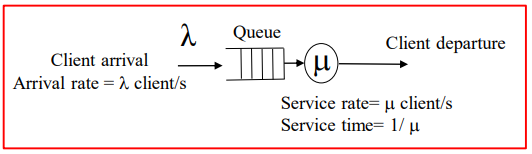
\includegraphics[width=7cm]{queue_model.png}
    \caption{Depiction of a queue model}
\end{figure}

\begin{itemize}
    \item Characterization of Delay - Important performance parameter in computer networks
    \item Customers (packet to be transmitted through a link) arrive at random times to obtain service (transmit a packet) 
\end{itemize}

\textbf{Important Variables and Expressions}
\begin{description}
    \item[\(\lambda\)] \hfill \\ arrival rate
    \item[\(\mu\)] \hfill \\ service rate
    \item[N] \hfill \\ Average number of customers/packets in the network
    \item[T] \hfill \\ Average delay per packet -> waiting plus service times 
    \item[\(\rho\)] \hfill \\ traffic intensity (occupation of the server)
    \item[\(T_{pac(frame)}\)] \hfill \\ Service time = packet transmission time
\end{description}

\begin{equation}
    T_{pac(frame)} = \frac{L}{C} = \frac{1}{\mu}
\end{equation}

\begin{equation}
    \rho = \frac{\lambda}{\mu}
\end{equation}

\subsubsection{M/M/1 Queue}

\begin{itemize}
    \item Poisson arrival
    \item Exponential service time
    \item Time Division Multiplexing
\end{itemize}

\textbf{Important Variables and Expressions}
\begin{description}
    \item[\(T_{W}\)] \hfill \\ average waiting time
    \item[\(N_{W}\)] \hfill \\ average number of clients waiting
\end{description}

\begin{equation}
    N = \frac{\rho}{1-\rho} = \frac{\lambda}{\mu-\lambda}
\end{equation}

\begin{equation}
    T = \frac{1}{\mu-\lambda}
\end{equation}

\begin{equation}
    T_{W} = T - T_{S} = \frac{1}{\mu-\lambda} - \frac{1}{\mu} = \frac{\rho}{\mu(1-\rho)}
\end{equation}

\begin{equation}
    N_{W} = T_{w}\lambda = \frac{\lambda}{\mu-\lambda} - \frac{\lambda}{\mu} = N - \rho
\end{equation}

\subsubsection{M/D/1 Queue}

\begin{equation}
    T_{W} = \frac{\rho}{2\mu(1-\rho)}
\end{equation}

\subsubsection{M/G/1 Queue}

\begin{equation}
    T_{W} = \frac{\lambda E(T_{pac(frame)}^2)}{2(1-\rho)}
\end{equation}

\end{document}